\documentclass[10pt]{article}
\usepackage[T1]{fontenc}
\usepackage[utf8]{inputenc}
\usepackage[margin=0.7in]{geometry}
\usepackage{graphicx}
\usepackage{booktabs}
\usepackage{amsmath}
\usepackage{amssymb}
\usepackage{array}
\usepackage{caption}
\captionsetup{font=small}
\usepackage[hidelinks]{hyperref}
\usepackage{titlesec}
\titleformat*{\section}{\large\bfseries}
\titleformat*{\subsection}{\normalsize\bfseries}
\setlength{\parskip}{0.15em}
\graphicspath{{./}{figures/}}

\title{\textbf{An Autonomous Agent that Derives ADC Linker Rules from the Literature, Designs the Molecules, and Flags When the Field Disagrees}}
\author{Elia Savino$^{1}$, Joshua W.\ Sin$^{2,3}$, Morgan G.\ L.\ Reigner$^{1}$, Miqu\`el \`A.\ P\'erez-Puigdom\`enech$^{2}$, Derk H.\ W.\ ten Klooster$^{1}$}
\date{}
\begin{document}
\maketitle
\begin{center}\footnotesize $^{1}$No\"el Research Group, Van 't Hoff Institute for Molecular Sciences, University of Amsterdam. $^{2}$Laboratory of Artificial Chemical Intelligence (LIAC), EPFL. $^{3}$Process Chemistry \& Catalysis, F.\ Hoffmann-La Roche AG, Basel.\end{center}
\begin{abstract}The right linker for an antibody conjugate depends on its payload: cytotoxins favour cleavable release, immune-stimulating conjugates demand plasma stability, and antibody--oligonucleotide conjugates were reported to need a rigid non-cleavable linker. We built an agent that reads 31 primary papers, derives a design rule per payload class with a retrieval-grounded language model, and lets each rule parameterise a REINVENT4 objective that then generates the linkers, so the delivered molecules carry the class motif by construction. A leave-one-paper-out test shows the cytotoxin and ISAC rules are robust---withhold a paper and the agent re-derives the same cleavable rule (confidence 0.97, 0.83)---while the ARC rule is contested: withholding the rigid-non-cleavable siRNA paper makes the agent derive the opposite rule, protease-cleavable Val-Cit, from the clinical antibody-oligonucleotide literature, and its confidence falls to 0.33 because the grounded evidence genuinely splits. The rule-generated Val-Cit design is recognised by cathepsin~B (predicted $K_\mathrm{d}$ 9\,nM) as tightly as the clinical substrate, while the rigid ARC design is not. Every reported value is provenance-tagged (a real model run, an LLM completion, or a cheminformatics heuristic) and a gate blocks any placeholder from a result---so the contested-ARC finding is a grounded, calibrated conclusion a lookup-table system could not produce.\end{abstract}
\begin{figure}[t]\centering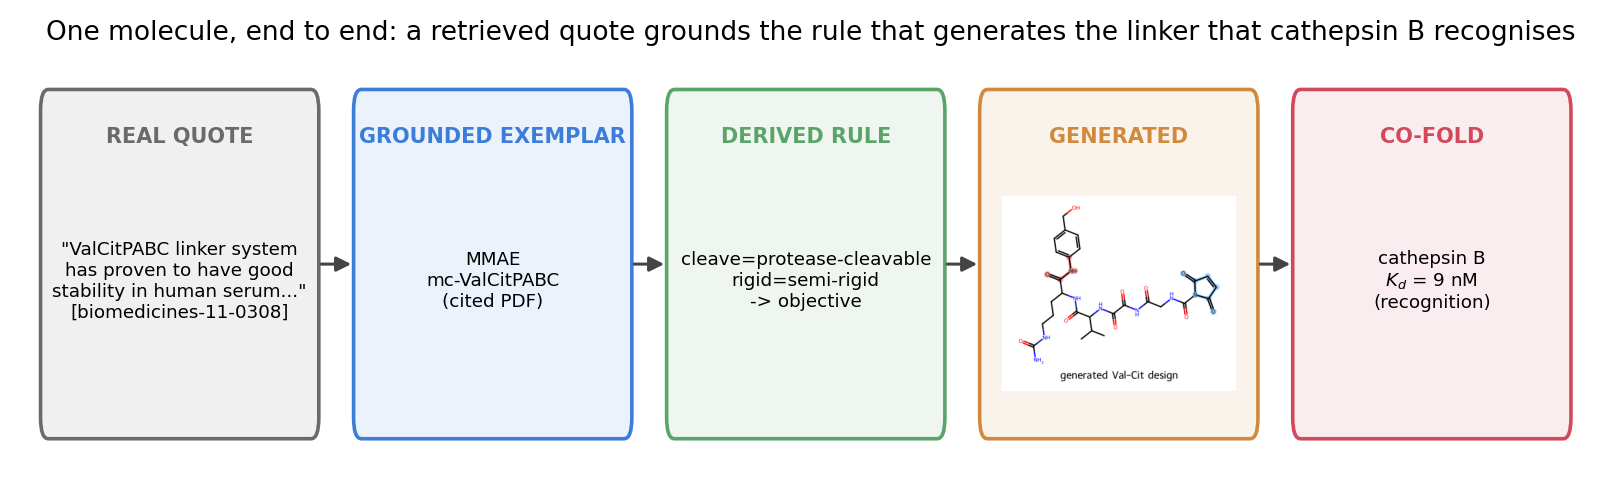
\includegraphics[width=0.98\linewidth]{fig1_journey.png}\caption{One molecule, end to end: a retrieved quote grounds the cytotoxin rule that generates a Val-Cit linker that cathepsin~B recognises. Handle (blue), scissile bond (red) and spacer (green) are SMARTS-detected.}\label{fig:journey}\end{figure}
\section{Introduction}Antibody conjugates couple antibody selectivity to a potent cargo, and the linker sets their therapeutic index~\cite{su2021,peng2021}. The linker requirement inverts with payload class: cytotoxins favour cleavable release~\cite{balamkundu2023}, ISACs demand plasma stability~\cite{isac2022,isac2025}, and antibody--oligonucleotide conjugates (ARCs) were reported to favour rigid non-cleavable linkers~\cite{arc2025}. An autonomous scientist should derive such rules from the literature, use them to design molecules, and report how confident it is---including recognising where the literature genuinely conflicts. We show all three, and the last surfaces a real, unresolved tension in ARC linker design (Figure~\ref{fig:journey}).
\section{Methods}\subsection{Reasoning that drives generation}
For each payload class an agent (Claude Opus, always on) queries a store of 31 papers, retrieves passages with provenance, and extracts conjugate exemplars that must each cite a retrieved passage. It derives a rule (cleavage, rigidity, plasma-stability) from the grounded exemplars---with no hardcoded fallback, so a failed call is an explicit abstain---and the rule compiles into an ADC goal profile (cleavage regime, rotatable-bond window, per-term weights) that parameterises the REINVENT4 LinkInvent objective. That objective then generates the linkers (staged learning, remote GPU); the class trigger warhead (Val-Cit-PABC, Val-Ala-PABC or the rigid sulfo-SMCC cap) is welded into every molecule (Figure~\ref{fig:steer}).

\subsection{Confidence, scorers and provenance}
Rule confidence is \emph{disagreement-aware}: it is high only when the grounded exemplars are both plentiful and consistent, so a split field drives confidence down and is flagged contested. Synthesizability is the continuous Ertl SA\_Score (the metric the generator optimises); the step-count survives only as a reported complexity index, not a route. Plasma stability is mechanism-resolved. Every value that reaches the manuscript is tagged \emph{measured} (a real Boltz or REINVENT run), \emph{llm}, or \emph{heuristic}; a gate blocks any placeholder from a results claim (SI provenance table).

\subsection{Held-out test and co-fold}
We withhold a class's key paper, re-derive the rule from the remaining corpus, record the prediction before revealing the withheld paper, and report agree/disagree with its evidence composition. We co-fold each designed linker with its real payload against cathepsin~B (Boltz-2) as two co-present ligands---a recognition/plausibility check, not a covalent conjugate and not a claim of cleavage.
\section{Results}\subsection{The rules generate, and steer, the molecules}
Each derived rule compiles into a distinct objective (Figure~\ref{fig:steer}, left) that generates its linkers: the designs separate cleanly by class along the two rule knobs (Figure~\ref{fig:steer}, right), ARC in a rigid non-cleavable region (4--6 rotatable bonds), cytotoxin and ISAC as cleavable flexible peptides (12--16). The molecules are made by the reasoning, not labelled after the fact.

\subsection{Held-out test: robust rules and a contested one}
The leave-one-paper-out test discriminates (Figure~\ref{fig:heldout}, Table~\ref{tab:heldout}). The cytotoxin and ISAC rules are robust: their grounded exemplars are unanimously cleavable, so withholding a paper leaves the derived rule and its high confidence intact. The ARC rule is contested. With the full corpus the top-retrieved siRNA papers give rigid non-cleavable. Withhold them, and from the clinical antibody-oligonucleotide literature (DYNE-101/251, AOC-1001) the agent derives protease-cleavable Val-Cit instead---its direction flips, and because the grounded evidence splits four cleavable to two non-cleavable, its disagreement-aware confidence falls to 0.33. Early cationic-assistance-free siRNA conjugates favour rigid non-cleavable linkers; clinical AOCs increasingly use cleavable Val-Cit. The agent surfaces that tension and lowers its confidence accordingly, rather than asserting a single rule.

\begin{table}[t]\centering\caption{Leave-one-paper-out. Confidence is disagreement-aware; ``evidence'' is the grounded cleavable/non-cleavable split. The ARC rule flips direction and loses confidence because its evidence is genuinely divided.}\label{tab:heldout}\small
\begin{tabular}{l l c c c l}\toprule
Class & Withheld & Full-corpus & Held-out & Evidence & Outcome \\ \midrule
Cytotoxin & Balamkundu 2023 & cleavable (0.60) & cleavable (0.97) & 8/0 & recovers \\
Immunomodulator (ISAC) & imidazoquinoline ISAC & cleavable (0.83) & cleavable (0.83) & 1/0 & recovers \\
Oligonucleotide (ARC) & ARC siRNA (Bioconj.\ Chem.\ 2025) & non-cleavable (0.50) & cleavable (0.33) & 4/2 & flips, contested \\
\bottomrule\end{tabular}\end{table}

\subsection{Structural recognition}
The rule-generated Val-Cit cytotoxin design co-folds tightly with cathepsin~B (predicted $K_\mathrm{d}$ 9\,nM), near the clinical mc-Val-Cit-PABC substrate (35\,nM), while the rigid non-cleavable ARC design binds an order of magnitude more weakly (109\,nM) (Figure~\ref{fig:cofold}). Affinity indexes recognition, not cleavage.

\subsection{Actionable designs}
Table~\ref{tab:short} gives one representative generated design per class (all fifteen, with dossiers---route, cost, failure modes, validation---in the SI). Structures are drawn with SMARTS-detected handle/scissile/spacer highlights (Figure~\ref{fig:journey}).
\begin{figure}[t]\centering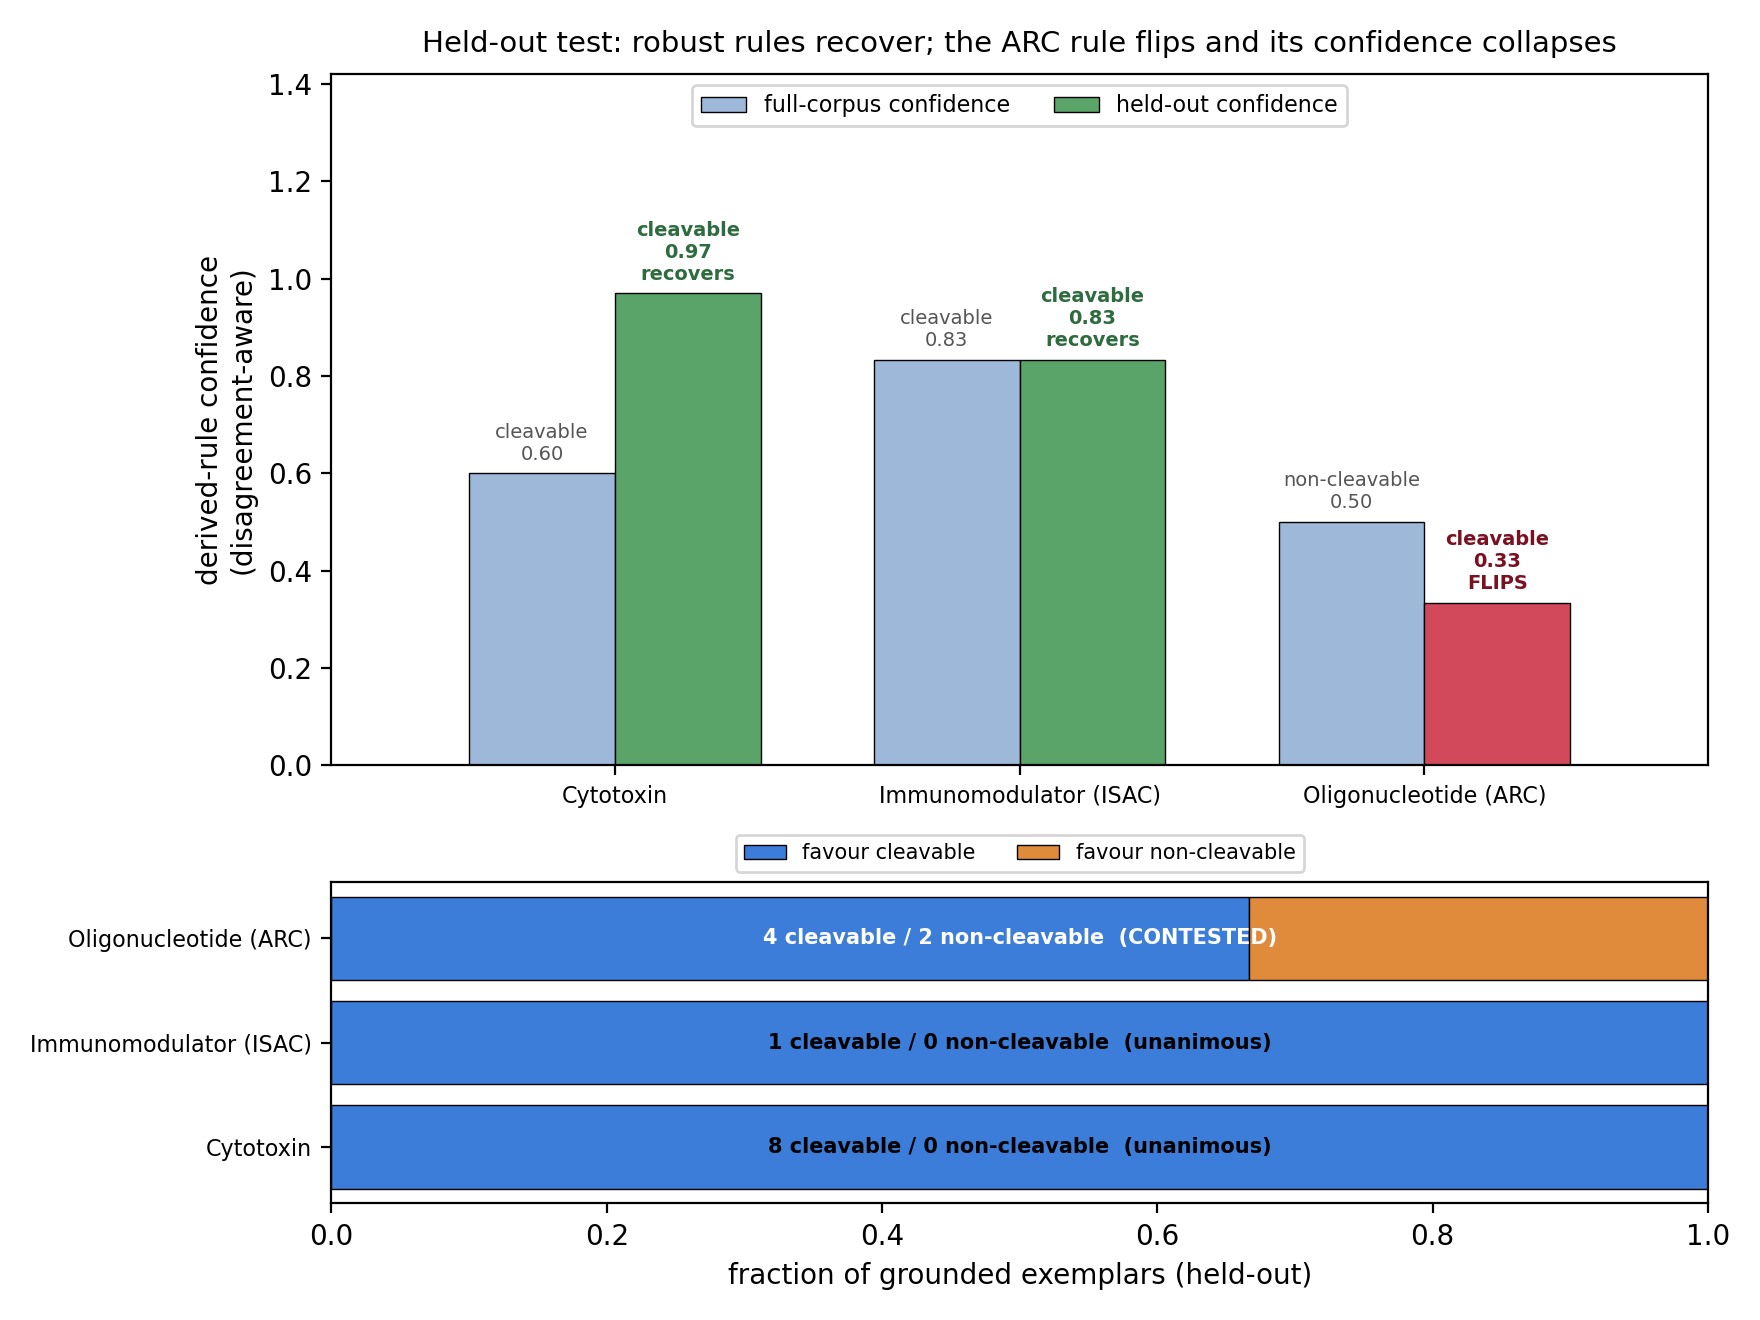
\includegraphics[width=0.86\linewidth]{fig2_heldout.png}\caption{Held-out test. Top: full-corpus vs held-out confidence (disagreement-aware); the ARC rule flips (red) while cytotoxin/ISAC recover (green). Bottom: the grounded-evidence split that explains it---ARC is 4:2 (contested), the others unanimous.}\label{fig:heldout}\end{figure}
\begin{figure}[t]\centering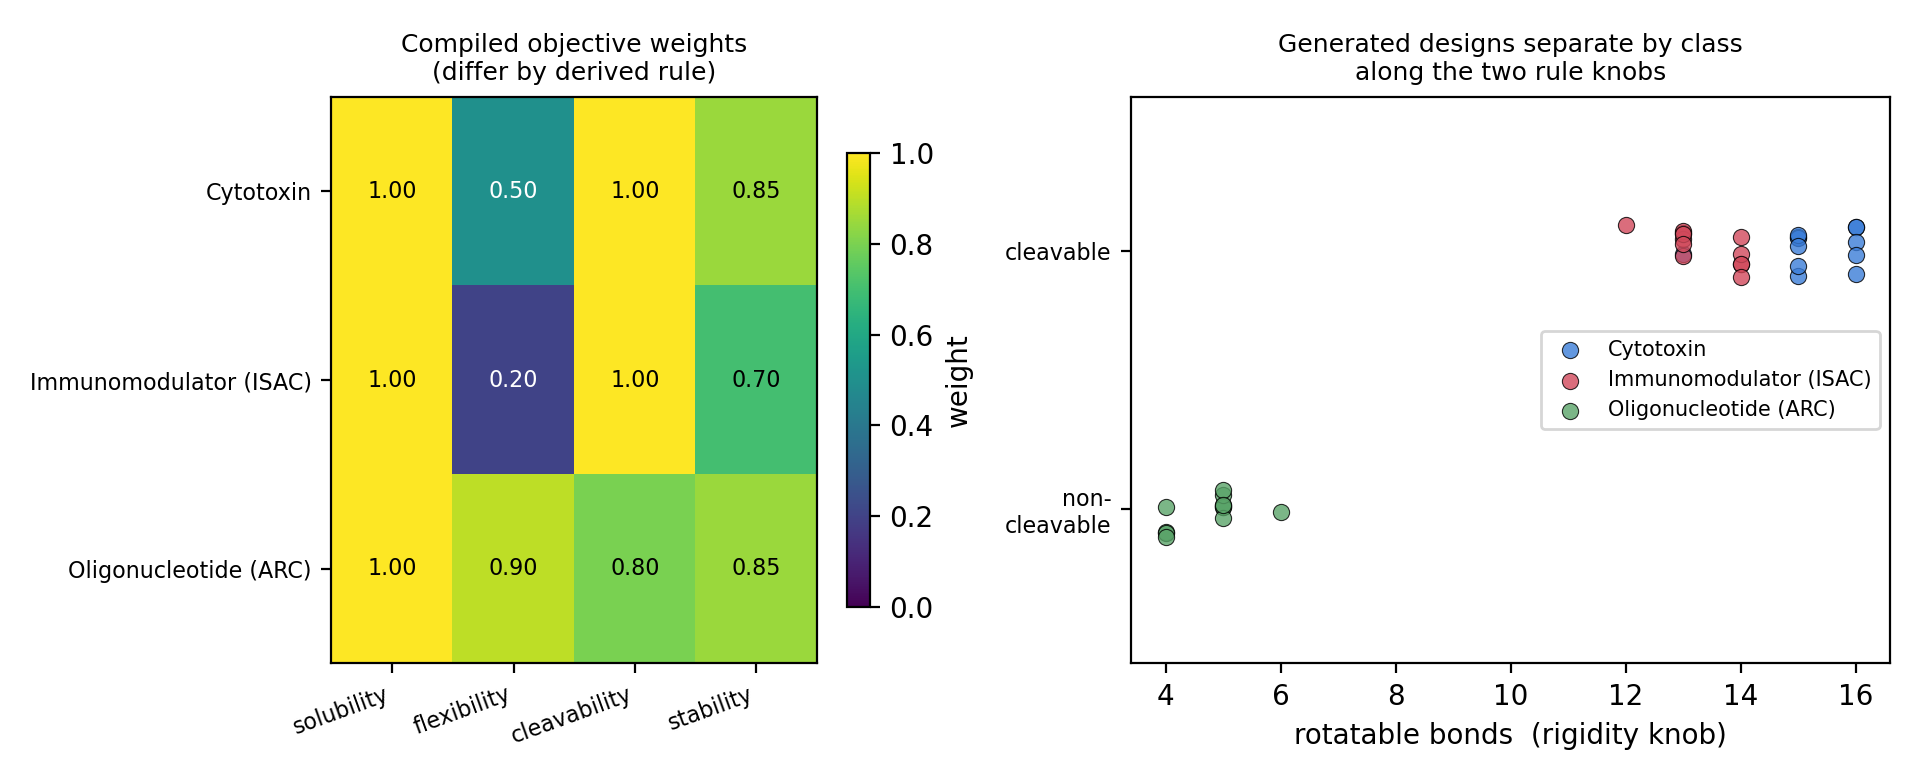
\includegraphics[width=0.98\linewidth]{fig3_rules_steer.png}\caption{The rules steer the chemistry. Left: the compiled objective weights differ by class. Right: the generated designs separate by class along the two rule knobs (rotatable bonds; cleavable-motif presence).}\label{fig:steer}\end{figure}
\begin{figure}[t]\centering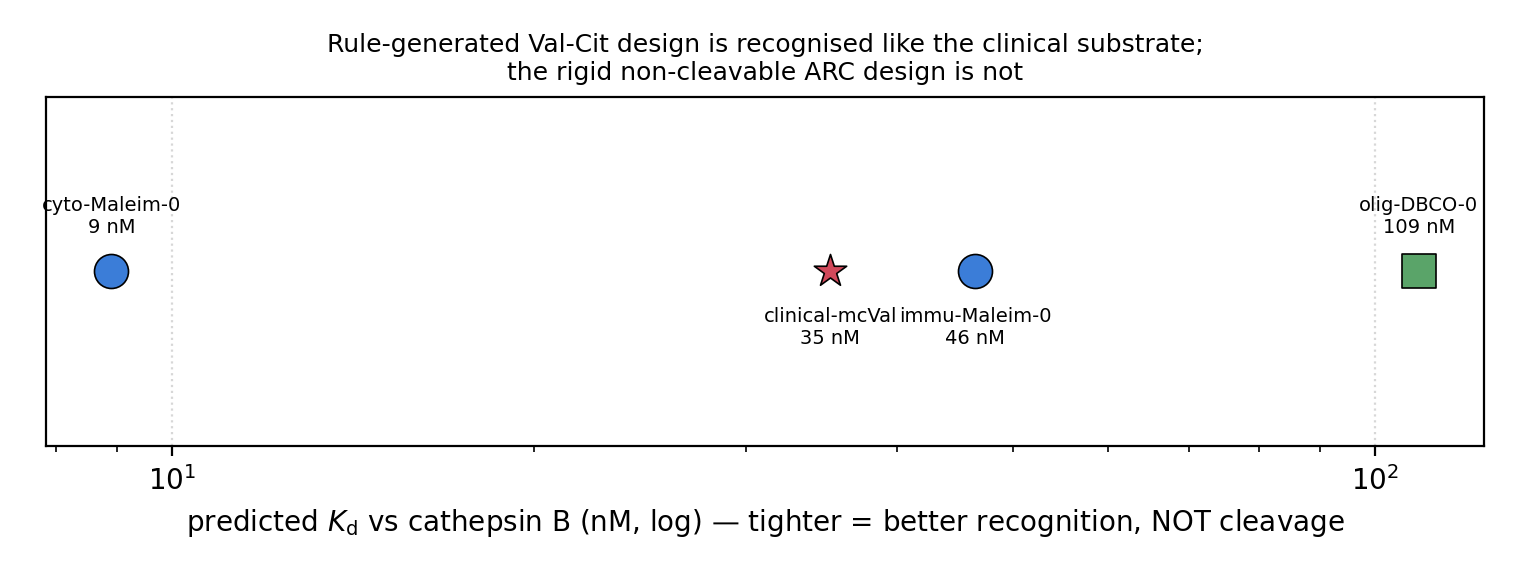
\includegraphics[width=0.72\linewidth]{fig4_cofold.png}\caption{Cathepsin-B co-fold. The rule-generated Val-Cit design binds as tightly as the clinical substrate; the rigid non-cleavable ARC design does not. Predicted affinity indexes recognition, not cleavage.}\label{fig:cofold}\end{figure}
\begin{table}[t]\centering\caption{One representative generated design per class (all fifteen with full dossiers in the SI). SA = continuous Ertl synthetic-accessibility subscore; Stab = mechanism-resolved plasma-stability score.}\label{tab:short}\small
\begin{tabular}{l l c c l}\toprule
Class & Representative generated linker & SA & Stab & Nearest clinical (Tc) \\ \midrule
Cytotoxin & \texttt{CC(C)C(NC(=O)C(=O)NC(=O)CNC(=\ldots{}} & 0.6437 & 0.85 & mc-Val-Cit-PABC (0.654) \\
Immunomodulator (ISAC) & \texttt{CC(NC(=O)C(NC(=O)CC(N)C(=O)NC\ldots{}} & 0.6547 & 0.85 & mc-Val-Ala-PABC (0.58) \\
Oligonucleotide (ARC) & \texttt{NCC1CCC(NC(=O)N2CCN(c3ccc(S(=\ldots{}} & 0.6866 & 1.0 & MCC (non-cleavable (0.145) \\
\bottomrule\end{tabular}\end{table}
\section{Discussion}The agent reads the literature, derives rules that generate synthesisable molecules, and reports calibrated confidence that falls when the evidence divides---turning ``contested'' from a caption into a computed output. The ARC result is the payoff: a grounded, non-obvious finding that clinical antibody-oligonucleotide conjugates favour cleavable Val-Cit, against the rigid-non-cleavable rule of the early siRNA literature. \emph{Limitations.} The complexity index is a count-based proxy, not a retrosynthetic route (AiZynthFinder is the planned upgrade); the co-fold places linker and payload as co-present ligands, not a covalent construct; the retrieval is lexical; and generation samples 25 designs per class. Each is tagged, not hidden.
\section{Conclusion}An autonomous agent derived payload-class ADC-linker rules from 31 papers, used them to generate synthesisable linkers, and, under a held-out test, distinguished robust rules from a genuinely contested one---surfacing an unresolved question in ARC linker design and lowering its confidence where the literature divides. The approach points toward an autonomous medicinal-chemistry scientist that designs and knows what it does not know.
\section*{Acknowledgements}
AI tools (Anthropic Claude) were used for retrieval-grounded literature reasoning, code, and manuscript drafting under author supervision. Per ICMJE and publisher policy, AI tools are not listed as authors; all scientific decisions and the final text are the authors' responsibility.
\begin{thebibliography}{9}
\bibitem{su2021} Su, Z.; et al. Antibody--drug conjugates: Recent advances in linker chemistry. \emph{Acta Pharm. Sin. B} \textbf{2021}, 11 (12), 3889--3907.
\bibitem{balamkundu2023} Balamkundu, S.; Liu, C.-F. Lysosomal-Cleavable Peptide Linkers in Antibody--Drug Conjugates. \emph{Biomedicines} \textbf{2023}, 11 (11), 3080.
\bibitem{peng2021} Peng, B.; et al. Stimulus-cleavable chemistry in controlled drug delivery. \emph{Chem. Soc. Rev.} \textbf{2021}, 50, 4737--4762.
\bibitem{su2021zhang} Su, D.; Zhang, D. Linker Design Impacts ADC Pharmacokinetics and Efficacy. \emph{Front. Pharmacol.} \textbf{2021}, 12, 687926.
\bibitem{arc2025} Antibody--siRNA conjugates for tumor cell gene silencing without cationic assistance. \emph{Bioconjugate Chem.} \textbf{2025}. DOI: 10.1021/acs.bioconjchem.5c00212.
\bibitem{isac2022} Immune-stimulating antibody conjugates elicit robust myeloid activation (TLR7/8 ISAC). \emph{Mol. Pharmaceutics} \textbf{2022}. DOI: 10.1021/acs.molpharmaceut.2c00392.
\bibitem{isac2025} Design of TLR7/8 agonist immune-stimulating antibody conjugates with tuned linker cleavability. \emph{J. Med. Chem.} \textbf{2025}. DOI: 10.1021/acs.jmedchem.5c01908.
\bibitem{boltz2} Passaro, S.; et al. Boltz-2: Towards accurate and efficient binding-affinity prediction. \textbf{2025}.
\end{thebibliography}

\end{document}